\documentclass{article}
\usepackage[utf8]{inputenc}
\usepackage[russian]{babel}
\usepackage{graphics}
\usepackage{amsfonts}
\usepackage{amssymb}

\ifx\pdfoutput\undefined
\usepackage{graphicx}
\else
\usepackage[pdftex]{graphicx}
\fi

\hoffset -2.0cm	
\voffset -3.0cm
\textheight 23.5cm 
\textwidth 17.0cm

\title{\bf Отчет \No 4}
\author{Амосов Федор}

\begin{document}
	\maketitle
	
	\paragraph{Введение}
        В данном отчете я рассмотрю основную часть построения VoR--Tree, а именно, построение графа Делоне (диаграммы Вороного) на данном наборе точек $P = \{p_i\}_{i = 1}^n$. 
    
        Вспомним наш рекурсивный алгоритм построения R--дерева. 
        \begin{itemize}
            \item На очередном шаге мы выбираем $S$ --- случайный небольшой поднабор $P$.
            \item Разбиваем все точки $P$ по клеткам Вороного набора $S$. Обозначим полученные наборы как $\{P_i\}_{i = 1}^m$. Соответствующие клетки обозначим за $\{C_i\}_{i = 1}^m$. Далее, мы будем опускать $\{\}_{i = 1}^m$.
            \item Строим R--дерево в каждой клетке Вороного.
            \item Подвешиваем все поддеревья за новую корневую вершину.
        \end{itemize}    
    
        Построение VoR--дерева будем проводить по той же схеме --- мы будем строить граф Делоне точно так же рекурсивно. Пусть мы построили $D_i$ --- граф Делоне для каждого набора $P_i$. Хочется научиться как--то <<склеивать>> полученные $D_i$ в один граф Делоне $D$ набора точек $P$. Далее, я представлю <<ход мыслей>> по поводу того, как это сделать.
    
    \paragraph{Склеивание выпуклых оболочек\\}
        \begin{itemize}
            \item Найдем $H_i$ --- все точки из набора, лежащие на границе выпуклой оболочки $P_i$.
            \item Построим граф Делоне точек $\cup_{i = 0}^m H_i$.
            \item Оставим в нем только ребра, которые соединяют вершины разных $P_i$. Обозначим оставшийся граф за $G$.
            \item Итоговый граф Делоне получится объединением $G$ и $D_i$.
        \end{itemize}
          Было бы отлично, чтобы полученный граф действительно был бы графом Делоне, но, к сожалению, это не так. Но об этом позже. Итак, что должно выполняться, чтобы это было правдой. Во--первых,
          
    \paragraph{Предложение\\}
        Выпуклые оболочки $P_i$ не пересекаются.
    \paragraph{Доказательство\\}
        $$
            \left.
				\begin{array}{c}
					P_i \subset C_i	\\
					C_i \textrm{--- выпуклое множество}
				\end{array}
			\right\}		
			\Longrightarrow 
			Conv P_i \subset C_i
	    $$
	    $C_i$ дизьюнктны, поэтому $Conv P_i$ так же дизьюнктны, ч.т.д. \\  
	    
    Во--вторых,
    
    \paragraph{Предположение 1\\}
        $D_i \subset D$, где $D$ --- <<истинный>> граф Делоне набора точек $P$.\\
        
    Очевидно, что без выполнимости этого предположения все поломается. Перед тем, как представить контрпример, вспомним следующий факт про граф Делоне. 
    \paragraph{Факт\\}    
        [окружность = многомерная сфера, треугольник = многомерный симплекс]    \\
        Описанная окружность треугольника графа Делоне не содержит внутри точек из набора. И наоборот. Если описанная окружность треугольника не содержит внутри точек из набора, то стороны треугольника являются ребрами графа Делоне. 
        
    Тем самым, для выполнения предположения 1, все описанные окружности около треугольников графа $D_i$ не должны содержать в себе точки графов $D_j$. Но это неправда. Контрпример легко строится   
     
    \begin{center}
	    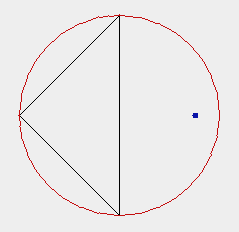
\includegraphics[scale = 0.5]{delaunay1.png}
	\end{center}           
	
	Где вершины треугольника принадлежат одной части $P_i$, а синяя выделенная точка --- другой части $P_j$ (и неважно, как построился граф $D_j$).
	
	Тем самым, <<склеивание выпуклых оболочек>> не работает. Если немного порисовать, то становится ясно, что треугольники на границе практически всегда <<залезают>> своими окружностями на соседние наборы. 
	
	Поэтому, придется какие--то треугольники перестраивать. Критерий очень простой --- надо перестроить только те треугольники, у которых окружности <<залезают>> на другие точки. Хочется что--то понять про то, сколько же таких <<плохих>> треугольников, которые надо будет перестроить. Ясно, что все такие треугольники расположены вблизи границ выпуклых оболочек $H_i$, потому что если окружность лежит целиком внутри $H_i$, то она никак не сможет <<залезть>> на другой набор в силу Предложения. После многочисленных рисунков, формируется следующее предположение,
	
	\paragraph{Предположение 2\\}
	    Если треугольник не находится на границе, то он <<хороший>>.\\
       
    Но и это тоже неверно. Для нахождения контрпримера надо порисовать чуть подольше, чем в первом случае,
            
	
	\begin{center}
	    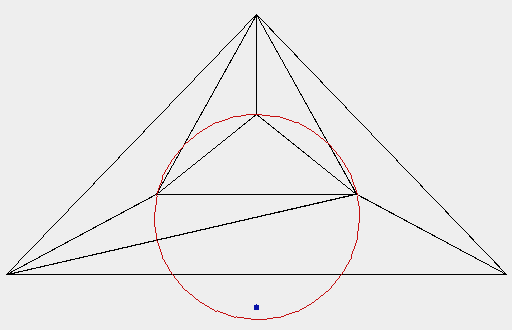
\includegraphics[scale = 0.5]{delaunay2.png}
	\end{center}
	
	Выделенная синяя точка снова принадлежит другой компоненте. И уже становится ясно, что нет никакого хорошего способа рассмотреть все <<хорошие>> треугольники. Поэтому, придется сделать что-нибудь не элементарное. 
	
	Итак, хочется найти все <<плохие>> треугольники не просматривая все треугольники. Для удобства назовем все пограничные треугольники тоже <<плохими>>. Рассмотрим $T$ --- граф соседних треугольников (два треугольника являются соседними, если у них есть общая {\bf вершина}). Каждая вершина $T$ --- это треугольник. Плохая вершина = плохой треугольник. 
	
	\paragraph{Утверждение\\}
	    Граф, индуцированный на плохие вершины $T$ связен.
	\paragraph{Доказательство\\}
	    Можно порисовать и все получится =)\\
	    
    После такого утверждения становится очевидной корректность следующего алгоритма поиска плохих треугольников,
    
    Делаем dfs на графе соседних треугольников только по плохим вершинам\\
    
        {\tt
            \noindent dfs(Triangle u) \{ \\
            \phantom ~~~~set u visited    \\
            \phantom ~~~~if ((u is <<good>>) and (u not on border)) \{    \\
            \phantom ~~~~~~~~return    \\
            \phantom ~~~~\}    \\            
            \phantom ~~~~add u to <<bads>>    \\ 
            \phantom ~~~~for v : neighbors of u \{   \\ 
            \phantom ~~~~~~~~if (v is not visited) \{    \\
            \phantom ~~~~~~~~~~~~dfs(v)    \\            
            \phantom ~~~~~~~~\}    \\
            \phantom ~~~~\}    \\
                     \}    \\
        }
      
    И запускаем от какого-нибудь крайнего треугольника.  
    	    
    	    
    	Остается только непонятным, как быстро проверить, есть ли в круге какие-нибудь точки. 
    	
    	Теперь алгоритм <<склеивания>> графов Делоне выглядит следующим образом. 
    	\paragraph{Склеивание выпуклых оболочек\\}
        \begin{itemize}
            \item Найдем для каждой $D_i$ по одному пограничному треугольнику.
            \item Запустим dfs от всех таких треугольников. Найдем все плохие треугольники.
            \item Построим граф Делоне на всех вершинах плохих треугольников.
            \item Оставим в нем только ребра, которые соединяют вершины разных $P_i$. В этом месте проблема. Обозначим оставшийся граф за $G$. 
            \item Итоговый граф Делоне получится объединением $G$ и $D_i$ без плохих треугольников.
        \end{itemize}
    	
    	Надо прикрутить MapReduce ко всему этому. Во--первых, граф Делоне для каждого $P_i$ можно строить на отдельной машинке. Во--вторых, запускать dfs для каждого $P_i$ можно тоже на разных машинках. Т.е. работать с компонентами независимо. Только слияние (последний пункт) придется сделать на одной главной машинке. Будем надеяться, что плохих треугольников будет мало, иначе главной машинке придется туго. Хотя, проклятие размерности все равно нам испортит весь праздник и перелопачивать придется практически все треугольники.          
	    
    \paragraph{Над чем нужно думать}
        \begin{itemize}
            \item Каким образом быстро определять пустоту круга? Видимо, нужен какой--нибудь дополнительный индекс. 
	        \item Какие ребра следует оставлять в графе $G$ в последнем алгоритме?
        \end{itemize}
        
	
\end{document}